\documentclass[a4paper,12pt,oneside]{letter}

\usepackage{ucs}
\usepackage[utf8x]{inputenc}
\usepackage[T1]{fontenc}
\usepackage{multicol}
\usepackage[english,francais]{babel}
\usepackage{fontenc}
\usepackage[pdftex]{graphicx}

\usepackage[pdftex=true,
hyperindex=true,
colorlinks=true,pdfstartview={Fit}]{hyperref}
\hypersetup{urlcolor=blue}


\usepackage{url}

\setlength{\parindent}{0cm} %Pour le retrait du paragraphe

\usepackage{soul} % Pour souligner ou barrer du texte
\usepackage{ulem}

\usepackage{textcomp}

\usepackage{setspace} % Interligne
\singlespacing
%\onehalfspacing
%\doublespacing

\usepackage{geometry}
\geometry{%
a4paper,
body={180mm,265mm},
left=15mm,top=15mm,
headheight=7mm,headsep=4mm,
marginparsep=4mm,
marginparwidth=11mm}

%\usepackage{eurosym}

%\usepackage{bookman} % Différents packs de police
%\usepackage{charter}
%\usepackage{newcent}
\usepackage{lmodern}
%\usepackage{mathpazo}
%\usepackage{mathptmx}



\usepackage{wrapfig} % pour encadrer les figures avec du texte

\usepackage{multicol} % Pour utiliser l'environnement multicol
\setlength\columnseprule{.4pt} % Pour mettre un trait séparateur de colonnes
\usepackage{multirow} % Pour fusionner les lignes dans les tableaux
\usepackage{array}
\usepackage{rotating} % Pour tourner un tableau
\usepackage{colortbl}
\usepackage{xcolor}



\date{2011-04-12}

\begin{document}

\begin{wrapfigure}[1]{r}{4.5cm}
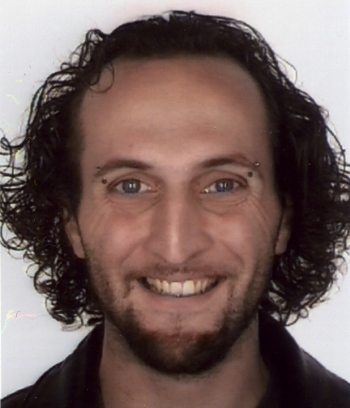
\includegraphics[width=4.5cm]{ID0.jpg}
\end{wrapfigure}

Name: GAU \hspace{1cm} Surname: Rémi \hfill

Sex: Male

Date of birth: 3\textsuperscript{rd} august 1982

Nationality: French

\begin{tabbing}
\hspace{3cm}\=\kill
Languages:
 \> French (mother tongue)\\ 
 \> English (bilingual)\\ 
 \> German (basics)\\ 
%  \> Norwegian (basics)
\end{tabbing}

{Tel (mobile):} (+33) 6 16 66 82 02

{Email:} \href{mailto:remi\textunderscore gau@hotmail.com}{remi\textunderscore gau@hotmail.com}


\begin{tabular}[!h]
{p{11cm}||p{7cm}}

\underline{\textbf{Address of last position:}} 									& \underline{\textbf{Secondary address:}}\\ 
\href{http://www.broca.inserm.fr/site_cpn/new/index.php}{Psychiatry and Neurosciences Center} (Site Pitié Salpêtrière) 	& 3 rue des troubadours\\
UMR - INSERM 894 - \href{http://www.upmc.fr/}{\textit{University Pierre et Marie Curie}} 				& Sur le Four\\
91 Boulevard de l’hôpital, 75 013 Paris, 										& 11 600 Malves en Minervois,\\
FRANCE 															& FRANCE \\
{Tel:} (+33) 1 40 77 97 14 												& {Tel:} (+33) 4 68 77 14 40
\end{tabular}

\setlength\minrowclearance{0.2cm}
\setlength\arrayrulewidth{2pt}

{%
\newcolumntype{A}{%
>{\bfseries}%
p{2.6cm}}

\newcolumntype{B}{%
>{\LARGE \centering \columncolor[gray]{.5}[.5\tabcolsep] \bfseries }%
p{17.6cm}}

\begin{tabular}{B}
\underline{ACADEMIC TITLES}
\end{tabular}

% \setlength{\fboxrule}{1pt}
% \framebox[18cm]{\LARGE\textbf{ACADEMIC TITLES}}

\begin{tabular}{Ap{14.5cm}}
\textbullet~\underline{2006-2010:} 	& \hfill \large\textbf{PhD in neurosciences} \hfill Defended in september 2010 \\ % Defended in september 2010 \\
					& \href{http://www.upmc.fr/}{\textit{University Pierre et Marie Curie}} (Paris, France) \newline
					  Doctoral School « \href{http://ed3c.snv.jussieu.fr/}{Cerveau, Cognition, Comportement} » \newline
					  first class honours \\
					& \large\underline{Thesis title:} Serotonergic neurons of the lateral paragigantocellular nucleus: roles in pain modulation and baroreflex inhibition \\
					& \underline{Laboratory:} \href{http://www.broca.inserm.fr/site_cpn/new/index.php}{Psychiatry and Neurosciences Center} \\
					& \underline{Supervisor:} BERNARD Jean-François \\
					& \underline{Email:} \href{mailto:jean-francois.bernard@upmc.fr}{jean-francois.bernard@upmc.fr} \hfill \underline{Tel:} (+33) 1 40 77 97 14
\end{tabular} 

\begin{center}
\Large\textbf{Graduate studies}
\end{center}

\begin{tabular}{Ap{14.5cm}}
\textbullet~\underline{2005-2006:} & \href{http://www.master.bip.upmc.fr/}{\large\textbf{Master of integrative biology and physiology, option: neurosciences – research specialization}} \newline
				     \normalsize \href{http://www.upmc.fr/}{\textit{University Pierre et Marie Curie}} (Paris, France) \newline
				     second class honours; rank: NA \\
\textbullet~\underline{2004-2005:} & \href{http://www.ups-tlse.fr/PANPS0_71/0/fiche___formation/&RH=rub02}{\large\textbf{Master of neuropsychology – research specialization}} \newline
				     \normalsize \href{http://www.ups-tlse.fr/}{\textit{University Paul Sabatier}} (Toulouse, France)\newline
				     second class honours; rank: NA \\
\textbullet~\underline{2003-2004:} & \large\textbf{Master of cellular biology and animal physiology} \newline
				     \normalsize \href{http://www.mcgill.ca/}{\textit{McGill university}} (Montréal, Canada) through the CREPUQ exchange program with the \href{http://www.univ-montp2.fr/}{\textit{University of Montpellier II}} (France)\newline
				     second class honours; rank: 1/55
\end{tabular} 

\pagebreak

\begin{center}
\Large\textbf{Undergraduate studies}
\end{center}

\begin{tabular}{Ap{14.5cm}}
\textbullet~\underline{2002-2003:} & \large\textbf{Licence of cellular biology and animal physiology} \newline
				     \normalsize \href{http://www.univ-montp2.fr/}{\textit{University of Montpellier II}} (France) \newline
				     second class honours; rank: 1/80 \\
\textbullet~\underline{2001-2003:} & \large\textbf{Diplôme d’études universitaires générales of psychology} \newline
				     \normalsize \href{http://www.univ-montp3.fr/}{\textit{University Paul-Valéry}} (Montpellier, France)\newline
				     second class honours; rank: NA \\
\textbullet~\underline{2000-2002:} & \large\textbf{Diplôme d’études universitaires générales of biochemistry and physiology} \newline
				     \normalsize \href{http://www.univ-montp2.fr/}{\textit{University of Montpellier II}} (France)\newline
				     first class honours; rank: 3/250
\end{tabular}


\begin{center}
\Large\textbf{Baccalaureate}
\end{center}

\begin{tabular}{Ap{14.5cm}}
\textbullet~\underline{2000:} & \large\textbf{International Baccalaureate} \newline
				\normalsize \href{http://www.rcnuwc.no/}{\textit{Red Cross Nordic United World College}} (Flekke, Norway) \newline
grade: 36/45 \\
\end{tabular}


\begin{tabular}{B}
\underline{CURRENT WORK}
\end{tabular}

My Phd was done in Professor Michel Hamon's team working on pain, stress and neurovegetative adaptations. This group is involved in several projects to study pain, its modulation and its associated autonomous responses by using different methods and models of acute and chronic pains. 

The largest part of the work of my PhD was focused on the \textit{in-vivo} single unit recording, in anesthetised rats, of neurons of the rostroventromedial medulla (RVM).
%, a region long known for its role in pain modulation, and especially its less studied lateral part: the lateral paragigantocellular nucleus (LPGi). 
This work aimed at showing that the numerous serotonergic (5-HT) neurons of this region are more heterogeneous and, in general, more responsive to noxious stimulation than was previously thought. 

This study involved a complete characterisation of the spontaneous activities of 5-HT neurons and of their reponses to innocuous as well as painful
%thermic and mechanic 
stimulations. This also involved an \textit{a posteriori} direct immunohistochemical identification of the neurotransmitter content of the recorded neurons using juxtacellular labelling and double immunofluorescence confocal microscopy. 

These recordings showed that a large majority of the 5-HT neurons of the RVM 
%and almost all of those found within the LGPi 
respond specifically to noxious stimuli. 
%Moreover, LPGi 5-HT neurons had more intense responses to nociceptive stimulation than those of 5-HT neurons found in the rest of the RVM.
Finaly, it was possible to differentiate subgroups of 5-HT neurons based on the correlation between their firing pattern at rest and the intensity of their responses to noxious stimuli, e.g 5-HT neurons with rapid, irregular firing at rest responded more to nociceptive stimulations.

This work also allowed to refine indirect algorithmic methods of identification of the 5-HT neurons based on their electrophysiological signature using linear discriminant analysis and to show the existence of “bursting” 5-HT neurons in this region.

Another part of the work my PhD involved various immunohistochemical techniques (neuroanatomical tracers, functional c-fos expression), as well as stereotatically directed pharmacological inactivation of RVM neurons combined with direct online cardiovascular parameters (heart rate, blood pressure) recording in anesthetized rats to assess the role of these neurons in cardiovascular regulations (GAU R., et al., Pain, 2009). 

These different lines of work allowed us to conclude that the general responsiveness of the 5-HT neurons of the RVM to noxious stimulation as well as their relative physiological heterogeneity argues in favor of their role, not only in pain modulation as was previously known, but also in the autonomic responses usually associated with noxious stimuli.


\begin{tabular}{B}
\underline{ACADEMIC APPOINTMENTS}
\end{tabular}

\begin{center}
\Large\textbf{Laboratory trainings}
\end{center}
\begin{minipage}[c]{7.7cm}
\textbullet~\underline{\textbf{2003-2005}}: In this laboratory, I was involved in two projects during my masters of animal physiology and neuropsychology.

\medskip

In the first, I conducted the data analysis of a pilot study preliminary to a multicentric rehabilitation program for dyslexic children.
\end{minipage}
\hfill
\begin{minipage}[c]{10cm}
\setlength\minrowclearance{0.2cm}
\setlength\arrayrulewidth{1.5pt}
\small
\begin{tabular}[t]{|l|}\hline
\underline{Laboratory:} Neuroimaging and neurological handicaps\\
INSERM unit 825, Hôpital Purpan, Toulouse, France\\
\underline{Supervisor:} DEMONET Jean-François\\
\underline{Email:} \href{mailto:jean-francois.demonet@inserm.fr}{jean-francois.demonet@inserm.fr}\\
\underline{Tel:} (+33) 5 61 77 95 19 \\ \hline
\end{tabular}
\end{minipage}

The study combined behavioral trainings (phonological and visuo-attentional in a cross-over design) to ameliorate the children's reading and fMRI experiments to evidence and explain reading improvements. 

This work aimed at evaluating the hypothesis that dyslexic children benefit more from a therapy when it is matched to the type of dyslexia they have (phonological versus visuo-attentional). 

Most of my work involved: 
\begin{enumerate}
\item modifying a lateral masking event-related fMRI paradigm designed for adults to use it with children, 
\item adapting part of the preprocessing (especially the normalisation) of the fMRI images to work with images from children and 
\item intra-subject statistical analysis of the effects of the different treatments on event-related fMRI data and their associated behavioral data.                                                                                                                                                                                                                                                                                                                                                                                                                 \end{enumerate}

To a lesser extend, I was also involved in the realisation and analysis of the broader neuropsycholinguistic evaluations of the children that were done before and after each treatment.

In the second project, I actively helped in the statistical analysis of both behavioral and PET neuroimaging data of experiments aimed at studying the categorical perception of phonemes in healthy and dyslexic adults. The correlational analysis between the subjects' in-scan behavioural responses and the intensity of the change in PET signal allowed us to identify brain regions whose activity during a phonological categorisation task differed the most between dyslexics and normal subjects.

During the time of my stay in the multidisciplinary research environement of this laboratory, I also became familiar, eventhough I did not use them personnaly with other neuroimaging and neuropsychological techniques and analyses, such as diffusion tensor tractography, EEG, TMS...

\pagebreak

\begin{tabular}{B}
\underline{OTHER WORK EXPERIENCES}
\end{tabular}

\begin{center}
\Large\textbf{Laboratory trainings}
\end{center}

\begin{minipage}[c]{6.7cm}
\textbullet~\underline{\textbf{2004:}}	I worked for a month on electrophysiology experiments aimed at better understanding the effects of dopamine on the long term potentiation (LTP) of pyramidal neurons in slices of rat prefrontal cortex.
\end{minipage}
\hspace{3mm}
\begin{minipage}[c]{\textwidth}
\setlength\minrowclearance{0.1cm}
\setlength\arrayrulewidth{1.5pt}
\small
\begin{tabular}[c]{|l|}\hline
\underline{Laboratory:} Laboratoire de biologie des processus adaptatifs\\
\href{http://www.upmc.fr/}{\textit{University Pierre et Marie Curie}}, Paris, France\\
\underline{Supervisor:} OTANI Satoru\\
\underline{Email:} \href{mailto:satoru.otani@snv.jussieu.fr}{satoru.otani@snv.jussieu.fr}\\ \hline
\end{tabular}
\end{minipage}

\begin{minipage}[c]{7.7cm}
\textbullet~\underline{\textbf{2003:}}	I worked for 2 months on a set of experiments testing the effects of prenatal stress or in-utero cocaine injection on learning in young rats and on hippocampic long term potentiation on rat brain slices.
\end{minipage}
\hspace{3mm}
\begin{minipage}[c]{\textwidth}
\setlength\minrowclearance{0.1cm}
\setlength\arrayrulewidth{1.5pt}
\small
\begin{tabular}[c]{|l|}\hline
\underline{Laboratory:} Laboratoire de plasticité cérébrale\\
CNRS-UMR 5102, \href{http://www.univ-montp2.fr/}{\textit{University of Montpellier II}}, France\\
\underline{Supervisor:} VIGNES Michel\\
\underline{Email:} \href{mailto:mvignes@univ-montp2.fr}{mvignes@univ-montp2.fr}\\ \hline
\end{tabular}
\end{minipage}

\begin{tabular}{B}
\underline{TEACHING EXPERIENCES}
\end{tabular}

\textbullet~\underline{\textbf{2nd semester 2009:}} 	Teaching assistant for human evolution classes of the preparatory program to paramedical training in the University Pierre et Marie Curie

Supervisors: A. AURENGO \& T. DARRIBERE; Contact: bureau 207 bis, 91 boulevard de l’hôpital, 

75 634 Paris, Tel: (+33) 1 40 77 95 77

\textbullet~\underline{\textbf{1rst semester 2005:}} 	Teaching assistant for psychophysiology classes of the undergraduate psychology program of the University Mirail-Toulouse II

Supervisor: BRETDIBAT Jean-Luc; Email: \href{mailto:bretdiba@univ-tlse2.fr}{bretdiba@univ-tlse2.fr}

\begin{tabular}{B}
\underline{SCHOLARSHIPS}
\end{tabular}

\begin{tabular}{Ap{14.5cm}}
\textbullet~\underline{2006-2009:} & Scholarship of the French ministry of research and technology \\
\textbullet~\underline{2001-2003:} & Scholarship of the French society for the study and treatment of pain \newline
				     (SFETD: \url{http://www.sfetd-douleur.org})
\end{tabular}

\begin{tabular}{B}
\underline{PUBLICATIONS}
\end{tabular}

\begin{center}
\Large\textbf{Peer reviewed papers}
\end{center}

\textbullet~GAU R, SEVOZ-COUCHE C, LAGUZZI R, HAMON M, BERNARD JF; Evidence for differential response to noxious stimulation among the serotonergic neurons of the rostral ventromedial medulla, \textit{J. Physiol}, in preparation

\textbullet~GAU R, SEVOZ-COUCHE C, LAGUZZI R, HAMON M; BERNARD JF; \href{http://www.painjournalonline.com/article/S0304-3959\%2809\%2900554-5/abstract}{Inhibition of Baroreflex by Nociception: A Key Role for Lateral Paragigantocellular Serotonergic Cells},\textit{ Pain}, 2009 Déc 5, 146 (3) : 315-24 ; DOI : 10.1016/j.pain.2009.09.018

\textbullet~BERNARD JF, NETZER F, GAU R, HAMON M, LAGUZZI R, SÉVOZ-COUCHE C; \href{http://onlinelibrary.wiley.com/doi/10.1002/cne.21532/abstract;jsessionid=5BCAA74755E291EB3D5A1BF64254181B.d01t02}{Critical role of B3 serotonergic cells in baroreflex inhibition during the defense reaction triggered by dorsal periaqueductal gray stimulation}, \textit{Journal of comparative anatomy}, 2008 Jan 1; 506(1): 108-21 ; DOI : 10.1002/cne.21532

\begin{center}
\Large\textbf{Posters}
\end{center}

\textbullet~BERNARD JF, SEVOZ-COUCHE C, HAMON M, GAU R; \href{http://www.abstractsonline.com/Plan/ViewAbstract.aspx?sKey=2ec7e761-d49a-463b-ac8f-add5cb56402d&cKey=445f7232-9ea5-4312-a569-8c9f7e8be066&mKey={3F846F23-E219-40A0-B790-DBC3F75684FD}}{Responses of lateral paragigantocellular and raphe magnus serotonergic neurons to noxious stimuli: a comparative reappraisal using juxtacellular recording}, 13\textsuperscript{th} world congress on pain; International association for the study of pain; Montréal (Québec, Canada), 2010, PW 205 

\textbullet~BERNARD JF, SEVOZ-COUCHE C, HAMON M, GAU R, Involvement of lateral paragigantocellular reticular serotonergic and non-serotonergic neurons in nociceptive processes, Annual meeting of the Society for neurosciences, Chicago, (Ilinois, USA), 2009, 361.10/BB36

\textbullet~GAU R, SEVOZ-COUCHE C, HAMON M, LAGUZZI R, BERNARD JF; Inhibition of cardiac baroreflex by intense noxious stimuli: a serotonergic mechanism involving the lateral paragigantocellular reticular nuclei; Annual meeting of the Society for neurosciences, Washington (D.C., USA), 2008, 174.22/NN22

\textbullet~BERNARD JF, SEVOZ-COUCHE C, HAMON M, LAGUZZI R, GAU R; Critical role of the B3 group in the baroreflex inhibition evoked by thermal noxious stimulation in the rat, Annual meeting of the Society for neurosciences, San Diego (California, USA), 2007, 724.24/MM1

\textbullet~BERNARD JF, NETZER F, GAU R, HAMON M, LAGUZZI R, SEVOZ-COUCHE C; Serotonergic neurons of B3 group: critical role in baroreflex inhibition during the defense reaction in the rat; Annual meeting of the Society for neurosciences, Atlanta (Georgia, USA), 2006, 356.9/AA9

\begin{center}
\Large\textbf{Talks}
\end{center}

\textbullet~GAU R; \href{http://www.sfetd-douleur.org/ModuleEventPublic/viewPresentation.phtml?about=rc\%2f2010\%2f10econgres\%2f10e-congre\%2fsession\%2f20101118-0845-20\%2f1015-62\%2f_container}{Implication du groupe sérotoninergique B3 dans le contrôle des circuits de la douleur et des réactions neurovégétatives associées}; 10\textsuperscript{th} congress of the French society for the study and treatment of pain (SFETD: \url{http://www.sfetd-douleur.org}), Marseille (France), 18\textsuperscript{th} november 2010

\begin{tabular}{B}
\underline{SKILLS}
\end{tabular}

\begin{description}
\item[\textbullet~Human neuroimaging (using SPM):] PET scan \& MRI images preprocessing and analyses (individual, group with fixed effects models, correlation analysis to in-scan or out of scan behavioral data) for both block and event-related designs.\\

\item [\textbullet~Softwares:] Proficient use \& knowledge of SPM (neuroimaging), Spike 2 (electrophysiology), Freehand (vectorial drawing), Photoshop, Latex, Microsoft/Open Office. Good use \& knowledge of different statistic analysis softwares (SPSS, statisticA, Statview, SigmaPlot), Image J and of GNU/Linux operating system. Some use \& knowledge MRIcrow, C/C++ \& Matlab programming, Presentation.

\item [\textbullet~Electrophysiology:] \textit{In vivo} extracellular recording combined coupled to juxtacellular labeling in halothane anesthetized rats, LTP protocols and associated pharmacological modulation on rat brain slices using intracellular recording in current clamp or extracellular recording with a multi-electrodes array. 

\item [\textbullet~Functional neuroanatomy:] Use of neuroanatomical tracers (Phaseolus, TMR, fluorogold), functional c-fos expression experiments, stereotaxic local pharmacological neuroinactivation combined with direct online physiological parameters (heart rate, blood pressure...) recording and analysis (using spike 2) in anesthetized rats. 

\item [\textbullet~Microscopy \& histology:] Total animal fixation with formalin \& brain extraction, general histological techniques (Cresyl violet, thionin), double immunohistochemical and immunofluorescent labeling, epifluorescent transmission and confocal microscope images acquisition and processing, some notions of in situ hybridization.

\end{description}
% 
% \begin{tabular}{B}
% \underline{OTHER INTERESTS}
% \end{tabular}
% 
% \begin{itemize}
% \item Skepticism, history \& philosophy of sciences, evolution
% \item Gender studies, sociology and political economy
% \item Rock climbing (bouldering and traditional), running, telemark skiing 
% \item Literature (science fiction) 
% \item Music (classical, jazz, blues, metal)
% \end{itemize}
% 
}%

\end{document}
